\documentclass[12pt]{article}
\usepackage{amsmath}
\usepackage{breakurl}
\usepackage[utf8]{inputenc}
\usepackage[titletoc,toc,title]{appendix}
\usepackage{float}
\usepackage{enumitem}
\usepackage{hyperref}
\usepackage{polski}

% images
\usepackage{graphicx}
\DeclareGraphicsExtensions{.pdf,.png,.jpg}
\graphicspath{ {./materials/} }

% listings
\usepackage{listings}
\usepackage[usenames,dvipsnames]{color}
\definecolor{listinggray}{gray}{0.9}
\definecolor{lbcolor}{rgb}{0.95,0.95,0.95}
\lstset{
backgroundcolor=\color{lbcolor},
    tabsize=4,    
%   rulecolor=,
    language=C,
        basicstyle=\scriptsize,
        aboveskip={1.5\baselineskip},
        columns=fixed,
        showstringspaces=false,
        extendedchars=false,
        breaklines=true,
        prebreak = \raisebox{0ex}[0ex][0ex]{\ensuremath{\hookleftarrow}},
        frame=single,
        numbers=left,
        showtabs=false,
        showspaces=false,
        showstringspaces=false,
        identifierstyle=\ttfamily,
        keywordstyle=\color[rgb]{0,0,1},
        commentstyle=\color[rgb]{0.026,0.112,0.095},
        stringstyle=\color[rgb]{0.627,0.126,0.941},
        numberstyle=\color[rgb]{0.205, 0.142, 0.73},
%        \lstdefinestyle{C++}{language=C++,style=numbers}’.
}
\lstset{
    backgroundcolor=\color{lbcolor},
    tabsize=4,
  language=C++,
  captionpos=b,
  tabsize=3,
  frame=lines,
  numbers=left,
  numberstyle=\tiny,
  numbersep=5pt,
  breaklines=true,
  showstringspaces=false,
  basicstyle=\footnotesize,
%  identifierstyle=\color{magenta},
  keywordstyle=\color[rgb]{0,0,1},
  commentstyle=\color{OliveGreen},
  stringstyle=\color{red}
  }
  
\lstdefinelanguage{JavaScript}{
  keywords={break, case, catch, continue, debugger, default, delete, do, else, finally, for, function, if, in, instanceof, new, return, switch, this, throw, try, typeof, var, void, while, with},
  morecomment=[l]{//},
  morecomment=[s]{/*}{*/},
  morestring=[b]',
  morestring=[b]",
  sensitive=true
}
  
\title{Indeksowanie przestrzenne źródeł danych strumieniowych w silniku strumieniowej materializowanej listy agregatów}
\author{
	  Pelczar Piotr\\
	  \small{\texttt{piotpel817@student.polsl.pl}}
	  \\[3ex]
	  Sikora Paweł\\
	  \small{\texttt{pawesik788@student.polsl.pl}}
	}
\usepackage{datetime}
\newdate{date}{09}{09}{2014}
\date{\displaydate{date}}
 
\begin{document}
\maketitle
 
\begin{abstract}
This paper describes test.
\end{abstract}

\renewcommand{\contentsname}{Contents}

\newpage
\tableofcontents

\newpage

\section{Wstęp}
\label{sec:intro}

Projekt zadany w ramach przedmiotu Teoria Przestrzeni Danych i Algorytmów zakładał:

\begin{itemize}[noitemsep]
  \item zapoznanie się z metodami indeksowania źródeł danych strumieniowych, na przykładzie danych pomiarowych pochodzących ze stacji paliw,
  \item stworzenie generycznego generatora danych emitującego zdarzenia na podstawie założonego modelu (charakterystyce), opisanego w sekcji \ref{sec:eventgenerator} odpowiadającemu strumieniowemu źródle danych \ref{stream-query-gorawski},
  \item zaproponowanie rozwiązania implementacji zmaterializowanej listy agregatów dla przeprowadzania obliczeń na strukturach danych w sekcji \ref{sec:implementation}.
\end{itemize}

Dodatkowo zostały rozpoznane opensourceowe rozwiązania w kontekście ich potencjalnego wykorzystania, część wiedzy zostało zebrane w sekcji \ref{sec:solutions}.

Praca oraz kody programów zostały opublikowane w serwisie GitHub:\\
\url{https://github.com/athlan/polsl-tpdia-event-generator}

Oprócz teoretycznej dywagacji, wykonano szereg testów, w tym praktyczne zastosowanie algorytmu MapReduce do agregacji dziennych statystyk dotyczących wpisów wybranych użytkowników umieszczanych w serwisie Twitter (podsekcja \ref{sec:mapreduce-implementation-twitter}). Celem zebrania statystyk jest określenie zasięgu użytkownika oraz probie ocenienia, jaki ma wpływ na innych użytkowników (ang. \emph{influcene}).

W serwisie Twitter użytkownicy zamieszczają około 6.000 wiadomości na sekundę, co daje ponad 518 milionów wiadomości dziennie. Obserwujemy tylko mały wycinek wiadomości, natomiast już do tak małej skali trzeba zaprzęc algorytm MapReduce. To obrazuje, ile danych dziennie danych gromadzonych jest w całym serwisie i z jakimi problemami ekstrakcji danych zmaga się firma Twitter.



\section{Generator zdarzeń}
\label{sec:eventgenerator}

	\subsection{Opis generatora zdarzeń}
Program przy pomocy wykresu zamieszczonego w bmp tworzy tablicę z danymi, która zawiera informację o ilości tankowań w danym dniu.    Program dzieli dobrę na ilość okresów czasów, ich ilość jest równa długości wykresu, natomiast wysokość odpowiada ilości tankowań w tym okresie. Następnie dane przekazywane są do programu, który emituje zdarzenia z danego okresu czasu w równych odstępach. Aplikacja została napisana w sposób by możliwe było podpięcie dużej ilości klientów emitujących dane.
	\subsection {ModelDataHolder}
Moduł "ModelDataHolder" odpowiada za przekształcenie pliku bmp do postaci listy tankowań w danych przedziałach czasu. W przypadku gdy na wykresie występują dwie lub więcej wartości dla ilości tankowań moduł wypisuje najniższą wartość.
\lstinputlisting[language=java]{articlesQuotes/DumpPlotDataFromBmp.java}

	\subsection{EventEmiter}
Moduł EventEmiter odpowiedzialny jest za przekształcenie danych dostarczonych przez moduł "ModelDataHolder" do postaci tablicowej. Następnie oblicza długość przedziałów czasowych oraz odstęp czasowy pomiędzy występowaniem tankowań w każdym przedziale czasowym. Po obliczeniu długości przedziałów czasowych i odstępów czasowych pomiędzy zdarzeniami w przedzialne, moduł przystępuje do generowania zdarzeń. 
\lstinputlisting[language=JavaScript]{articlesQuotes/EventEmitter.js}

	\subsection{EventReceiver}
Moduł "EventReceiver" nasłuchuje i sprawdza wystąpienia tankowań generowanych przez moduł EventEmiter. Przy każdy nowym zdarzeniu moduł "EventReceiver" wykonuje akcje zapisaną w funkcji:
\lstinputlisting[language=JavaScript]{articlesQuotes/sample-client.js}
Istnieje możliwość podłączenie większej ilość modułów "EventReceiver".

	\subsection{}


\section{Zmaterializowana lista agregatów}

Aby poradzić sobie z przetwarzaniem większej ilości danych w ramach systemu zarządzania bazą danych stosuje się podejścia umożliwiające skalowanie horyzontalne oraz agregowanie danych. Dla rozwiązań z dużą ilością danych istnieją konkurencyjne rozwiązania do przeprowadzania obliczeń dla zapytań kierowanych bezpośrednio do silnika relacyjnej lub nierelacyjnej bazy danych.

\subsection{Algorytm Map-Reduce}
\label{sec:mapreduce}

MapReduce to podejście do przetwarzania ogromnych zbiorów danych w rozproszonych klastrach komputerowych\cite{google-map-reduce}. Stworzone przez Google rozwiązanie ma przewagę nad przetwarzaniem danych wewnątrz systemu bazodanowego, ponieważ umożliwia wykonywanie obliczeń na węzłach (w szczególności na klastrze komputerowym).

Podejście opłaca się, jeżeli infrastruktura zapewnia szybki przepływ informacji oraz wysoką odporność na błędy.

Model zakłada dwie fazy opisane w podsekcjach (oraz fazę pośrednią).

\subsubsection{Faza Map}
\label{sec:mapreduce-map}

Główny węzeł przyjmuje dane i definiuje podproblemy, które są wysyłane do innych węzłów. Inne węzły mogą ponownie wykonać fazę Map, zgodnie z logicznym połączeniem, dostępnymi zasobami, na zasadzie struktury drzewiastej. Gdy problem zostaje rozwiązany, informacja z rozwiązaniem pokonuje tę samą ścieżkę z powrotem w fazie Reduce (\ref{sec:mapreduce-reduce}), aż do głównego węzła.

Faza map wykorzystuje funkcję mapowania odwzorowującą klucz na wartość. W rezultacie, po kilku wywołaniach funkcji mapowania w fazie uzyskuje się listę wartości pogrupowaną wg klucza.

\subsubsection{Faza Shuffle}
\label{sec:mapreduce-shuffle}

Faza Shuffle przydziela klcuze węzłom rozpoczynającym fazę Reduce (\ref{sec:mapreduce-reduce}), nad którymi powinny 
pracować. Zapewnia, że praca jest równo rozłożona pomiędzy węzły przez cały czas trwania procesu.

\subsubsection{Faza Reduce}
\label{sec:mapreduce-reduce}

Główny węzeł oraz podwezły, które rozpoczęły fazę map zbierają odpowiedzi ze wszystkich podproblemów i formują je, aby udzielić finalnej odpowiedzi. W końcu, odpowiedzi trafiają do głównego węzła, który odpowiada wynikiem operacji.

W fazie Reduce wykorzystywana jest funkcja redukująca, która jako argumenty otrzymuje klucz oraz listę wartości związanych z danym kluczem. Zadaniem funkcji redukującej jest przekształcenie listy wartości w pojedynczą wartość. Wartości w liście przekazanej jako argument, mogą pochodzić z poprzedniej iteracji fazy Reduce (tj. jako wyniki funkcji redukujących) lub z warunków początkowych z fazy Map. W ten sposób można powielać fazę Reduce, dopóki odpowiedź nie zostanie udzielona w postaci pojedynczej wartości, a nie listy wartości skojarzonej z kluczem.

\subsubsection{Implementacja Map-Reduce na przykładzie bazy danych MongoDB oraz agragacji danych z portalu Twitter}
\label{sec:mapreduce-implementation-twitter}

Autor Piotr Pelczar pracował nad agregacją danych dotyczących statystyk kont w serwisie Twitter. Każdy wpis w serwisie Twitter jest reprezentowany jako pojedynczy dokument w dokumentowej bazie danych. Dany wpis może być komenatrzem do innego wpisu (\emph{comment}), wzmianką o autorze (ang. \emph{mention}) lub przekazaniem wiadomości dalej (\emph{retweet}).

Z API serwisu Twitter gromadzone są wszystkie wpisy, które są wzmiankami na temat danego autora, przekazaniem jego wiadomości dalej, są wiadomością jego autorstwa lub komentarzem pod nią.

Zadaniem programu jest policzenie, ile dziennie autor posiada wzmianek, komentarzy pod swoimi wpisami lub przekazania wiadomości dalej. Celem zebrania statystyk jest określenie zasięgu użytkownika oraz próbie ocenienia, jaki ma wpływ na innych użytkowników (\emph{influcene}).

\lstinputlisting[language=JavaScript]{./materials/mapreduce-nodejs-mongodb.js}

Definiujemy dwie fazy map:

\begin{itemize}[noitemsep]
  \item Pierwsza iteruje po wpisach dotyczących autora, wśród nich są komentarze pod jego wpisami oraz wzmianki.
  \item Druga iteruje po wpisach, które są przekazaniem wiadomości autora dalej przez innych użytkowników.
\end{itemize}

Faza Map tworzy obiekt z trzema polami: ilością komentarzy, liczbą wiadomości, które zostały przekazane dalej oraz ilością wzmianek. W funkcji map problem jest definiowany jako inkrementowanie wartości pól obiektu w zależności od typu wpisu. Obiekt statystyk jest mapowany na dziedzinę, czyli dane wpisy grupowane są po dniu. Znacznik czasowy dnia stanowi klucz.

Następnie w fazie Reduce wszystkie liczniki przyporządkowane do tej samej daty (mające wspólną wartość dziedziny, czyli klucza) są sumowane. W odpowiedzi otrzymujemy listę zsumowanych statystyk, zgrupowane po dniu.

\subsection{Agregowanie strumieniowych danych}

W nawiązaniu do Contineous Query Language (CQL)\cite{stream-query-gorawski}, operatorowi strumień-relacja o oknie czasowym \cite{stream-query-stanford-stochmialek}\cite{stream-processing-streamsql} oraz agregacji danych w oknach czasowych zostały znalezione rozwiązania, które realizują funkcjonalności przy założeniu, że wyznaczanie przedziału czasowego odbywa się jednokrotnie, a czas jest stały.

Rozpoznane zostały 


\section{Przegląd dostępnych rozwiązań dostępnych na rynku}
\label{sec:solutions}



\subsection{Hadoop}
\label{sec:solutions:hadoop}



\subsection{Hive}
\label{sec:solutions:hive}
Apache Hive to projekt, który umożliwia tworzenie kwerend i zarządzanie dużym zbiorem danych znajdujących się w pamięci rozproszonej. Hive wykorzystuje prosty język zapytań podobny do języka SQL. Język ten nazwany został QL. Język ten umożliwia tworzenie zapytań podobnych do zapytań SQL i umożliwia tworzenie własnych funkcji mapujących i redukujących przez użytkowników, którzy znają framework Map/Reduce. Język QL wykorzystywany przez Hive może być rozszerzony przez funkcje skalarne(UDF), agregujące (UDAF) i funkcje tablicowe (UDTF).

Apache Hive posiada:
\begin{itemize}[noitemsep]
\item narzędzia ułatwiających proces ETL,
\item mechanizm do przetwarzania różnych formatów danych,
\item zapytania wykonywane przy pomocy Map/Reduce
\end{itemize}

Hive nie oferuje przetwarzania zapytań w czasie rzeczywistym i aktualizacji wierszy o niskim narzucie czasowym. Hive najlepiej wykorzystać do dużych zbiorów danych, które ciągle napływają. Największymi zaletami Hive są:
\begin{itemize}[noitemsep]
\item skalowalność (skaluje się poprzez dodanie dodatkowych dynamicznych klastrów do Hadoop)
\item rozszerzalność ( MapReduce framework, UDF/UDA/UDTF)
\item tolerancja błędów
\end{itemize}
Hive zawiera HCatalog i WebHCat. HCatalog jest warstwą zarządzającą tabelami i pamięcią dla Hadoop, która możliwa użytkownikowi korzystać z różnych narzędzi do przetwarzania danych (np. MapReduce) w celu łatwiejszego odczytu i zapisu danych. WebHCat oferuje usługi, które umożliwiają uruchomienia na Hadoop'ie MapReduce, zadań Hive lub wykonać operację metadanową za pomocą protokołu HTTP(REST).


\subsection{Spark (Stream Spark)}
\label{sec:solutions:spark}

Apache Spark to projekt, którego częścią jest Apache Spark Streaming, czyli framework, który umożliwia przetwarzanie strumieniowych, stale napływających o dużej częstotliwości danych w czasie rzeczywistym. Dane mogą pochodzić z różnych źródeł, takich jak Kafka, Flume, ZeroMQ, czy natywne gniazda TCP (czyli implementacja zaproponowana w \ref{sec:eventgenerator-eventreceiver}). Przetworzone dane mogą być składowane na dysku, w bazach danych, wysyłane na szyny danych. Spark dostarcza również wbudowane algorytmy uczenia maszynowego (ang. \emph{machine learning}) oraz analizowania grafów (ang. \emph{graph processing}). Dane są definiowane pojęciem RDD\cite{manual-apache-spark-streaming} i nie zmieniają swojego stanu (\emph{immutable state}).

\begin{figure}[h!]
  \centering
    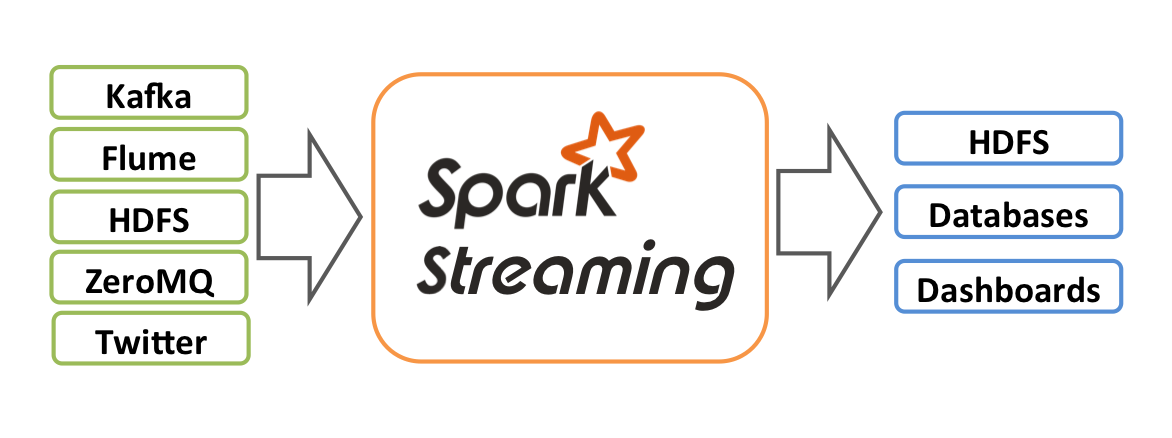
\includegraphics[scale=0.75]{spark-streaming-arch.png}
  \caption{Zasada działania Apache Spark Stream}
  \label{fig:spark-streaming-arch}
\end{figure}

Apache Spark Streaming umożliwia również obliczenia na przesuwnym oknie RDD:

\begin{figure}[h!]
  \centering
    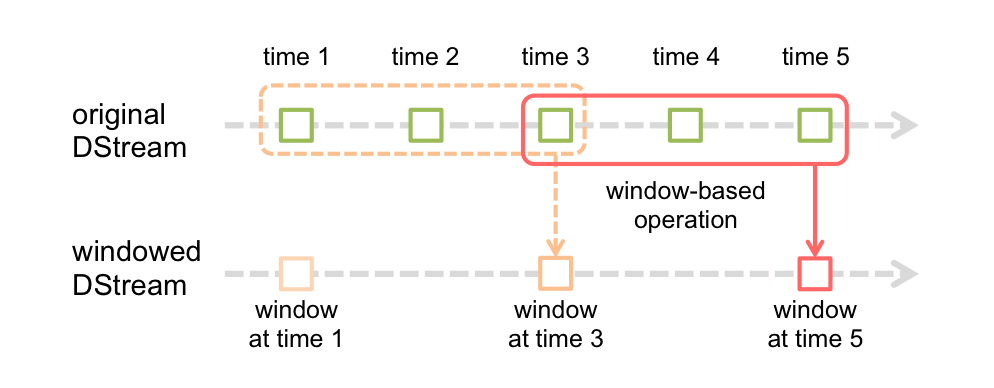
\includegraphics[scale=0.75]{spark-streaming-dstream-window.png}
  \caption{Przesuwne okno czasowe w Apache Spark Streaming}
  \label{fig:spark-streaming-dstream-window}
\end{figure}

Wykorzystanie Spark Streaming umożliwia wykonywanie operacji na strumieniu danych znanych z MapReduce oraz strumieniowych baz danych, w szczególności:

\begin{itemize}[noitemsep]
  \item map
  \item reduce
  \item filter
  \item transform
  \item union - złączenie źródeł danych
  \item count oraz countByValue
\end{itemize}


\section{Implementacja}
\label{sec:impl}

\subsection{Zmaterializowana lista agregatów}
\subsubsection{Pojęcie agregatu}
\label{sec:impl-mal-aggregate}

Na potrzeby projektu zostało zdefiniowane pojęcie agregatu\cite{mal-lru-gorawski} jako obiektu który zawiera jednostkę informacji skojarzoną z danym kluczem. Inaczej mówiąc, jednostka informacji jest rozumiana jako zgrupowana wartość według klucza.

Rozpatrujemy listę zmaterializowanych agregatów dla przestrzennego klucza temporalno-czasowego, których kluczem jest identyfikator miejsca (\emph{venueId}) oraz znacznik czasowy (\emph{timestamp}) wyrównany do okna czasowego (np minuty, godziny, dnia, miesiąca, roku)\footnote{Poprzez wyrównanie stempla czasowego do godziny mamy na myśli stempel czasowy pierwszej sekundy danej godziny, dla roku pierwszą sekundę pierszego dnia itd.}.

Zostały zdefiniowane następujące struktury w języku Java:

\begin{itemize}[noitemsep]
  \item \emph{IAggregateKey} - klucz agregatu, obiekt immutable (klucz może być złożony),
  \item \emph{IAggregateValue} - wartość agregatu, obiekt immutable (wartość agregatu może składać się z wielu pól),
  \item \emph{Aggregate} - zmaterializowany agregat, obiekt immutable (połączenie klucza z wartością).
\end{itemize}

\lstinputlisting[language=java]{../MaterializedAggregationFramework/src/pl/polsl/tpdia/mal/IAggregateKey.java}

\lstinputlisting[language=java]{../MaterializedAggregationFramework/src/pl/polsl/tpdia/mal/IAggregateValue.java}

\lstinputlisting[language=java]{../MaterializedAggregationFramework/src/pl/polsl/tpdia/mal/Aggregate.java}

\subsection{Mapowanie danych na agregaty}

Każda porcja informacji (krotka) napływająca strumieniowo, która trafia do systemu ma ściśle okrśloną strukturę, tj. klucz oraz zestaw wartości. Jednocześnie każda krotka sama w sobie jest agregatem (wartością atomową). Zdefiniowane zostały interfejsy pozwalające mapować agregaty na inne agregaty nazywane Mapperami (\emph{IAggregateMapper}).

Mappery przekształcają agregat w agregat o tych samych wartościach, lecz o zmienionym kluczu. Intencją jest zmmieniona granulacja klucza agregatu, na przykład implementacją mapera może być przekształcenie klucza krotki na wyrównany co do miesiąca, aby produkotwać krotki o wartościach pogrupowanych po miesiącu.

\lstinputlisting[language=java]{../MaterializedAggregationFramework/src/pl/polsl/tpdia/mal/IAggregateKey.java}

\subsection{Mappery oraz struktura agregatów}

Mapery mogą zostać połączone w łańcuch (\emph{Mapper Chain}), tak, aby dana krotka została zamapowana na wszystkie możliwe (w zależności od kontekstu, w jakim został zbudowany łańcuch) granulacje. Przykładowo istnieje możliwość połączenia Mapperów w łańcuch tak, aby wartość atomowa została przekształcona na agregat minutowy, następnie agregat minutowy na godzinowy, następnie agregat godzinowy na dniowy, itd. Produkowanie agregatów w łańcuchu prezentuje schemat \ref{fig:impl-mapping-chain}

\begin{figure}[h!]
  \centering
    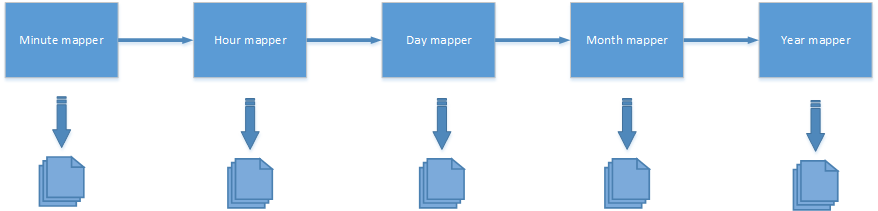
\includegraphics[scale=0.65]{impl-mapping-chain.png}
  \caption{Zasada łączenia Mapperów w łańcuch}
  \label{fig:impl-mapping-chain}
\end{figure}

\lstinputlisting[language=java]{../MaterializedAggregationFramework/src/pl/polsl/tpdia/mal/IAggregateMapper.java}

Agregaty logicznie ułożone są w kompozycję przypominającą dynamicznie tworzoną strukturę drzewiastą wg klucza. Fizycznie nie ma między nimi żadnych powiązań (referencji), a źródło danych, w którym utrwalane są agregaty, może być odpytywane punktowo.

\subsection{Tworzenie agregatów i procesor zapytań}

Każda porcja informacji, kótra trafia do systemu, zamieniana jest na agregat i iterpretowana jako wartość atomowa. Operacja ta ma na celu narzucenie struktury porcji informacji, czyli klucza oraz zestawu wartości. W ten sposób tworzone są pierwsze agregaty.

Zapytania zadane systemowi są przekazywane \emph{Procesorowi zapytań}, który rozbijane je na 4 fazy:

\begin{itemize}[noitemsep]
  \item analiza semantyczna zapytania,
  \item na podstawie łańcucha maperów zaplanowanie wszystkich możliwie największych agregatów, z których można złożyć odpowiedź
  \item kaskadowe zbieranie wyników ze wszystkich istniejących agregatów oraz (jeżeli nie istnieją) tworzenie nowych, wcześniej zaplanowanych agregatów, z wyników pośrednich,
  \item złączenie wyników z możliwie największych agregatów i udzielenie odpowiedzi
\end{itemize}

Agregaty mogą być tworzone w dowolnych momentach, a w szczególności:

\begin{itemize}[noitemsep]
  \item w momencie pojawienia się krotki w systemie\footnote{Podobnie jak struktury indeksujace w bazach daych} lub,
  \item przy pierwszym zapytaniu lub,
  \item w zależności od charakterystyki i obciążenia systemu (np jest więcej zapisów, niż odczytów), obliczanie agregatów może zostać opóźniane
\end{itemize}

Za wyliczenie agregatów odpowiedzialny jest mechanizm Reducera, który przyjmuje jako argumenty wjściowe klucz, po którym agregowane dane oraz listę wartości do agregacji. Jako wynik zwraca nowy agregat.

\lstinputlisting[language=java]{../MaterializedAggregationFramework/src/pl/polsl/tpdia/mal/IAggregateReducer.java}

\subsubsection{Sposób wyznaczania tworzenia agregatów przez procesor zapytań}

Gdy do systemu trafia zapytanie zakresowe po kluczu \emph{IAggregateKey} o wyliczenie wartości bazjąych na \emph{IAggregateValue} procesor zapytań analizuje zakres zapytania i na podstawie łańcucha mapperów przygotowuje listę wszystkich możliwie największych agregatów, które mogą zostać wykorzystane do zwrócenia wyniku zapytania.

\textbf{Przyład}

Przyjmujemy założenie, że agregacja informacji następuje po miejsach (\emph{venueId}) oraz po dacie wyrównanej do: roku, miesiąca, dnia, godziny, minuty. Jeżeli zostaje zadane zapytanie zakresowe od 2014-09-24 do 2014-11-05, wyznaczane są następujące możliwie największe agregaty:

\begin{itemize}[noitemsep]
  \item dzienne od 2014-09-24 do 2014-09-30,
  \item miesięczne od 2014-10-01 do 2014-10-31,
  \item dzienne od 2014-11-01 do 2014-11-05,
\end{itemize}

\subsubsection{Drążenie danych - wyznaczanie nieistniejących agregatów}
\label{sec:impl-mal-computing-aggregates}

Jeżeli agregaty, o które system został zapytany jeszcze nie istnieją w trwałym źródle danych, dekomponowane są na możliwie największe podagregaty (\emph{drążenie danych}). Jeżeli któreś podagregaty są już wcześniej obliczone, nie ma potrzeby ich ponownej dekompozycji, natomiast dla podagregatów, które nie są policzone proces powtarza się, aż proces dekompozycji sięgnie danych źródłowych, które są agregatami atomowymi.

Schemat działania zobrazowany jest na rysunku \ref{fig:impl-aggregate-chunking}.

\begin{figure}[h!]
  \centering
    
\includegraphics[scale=0.65]{impl-aggregate-chunking.png}
  \caption{Dekomponowanie agregatów oraz drążenie danych. Zielone kwadraty oznaczają obliczone pola, szare nieistniejące, pomarańczowym kolorem oznaczone zostały agregaty atomowe, czyli dane źródłowe}
  \label{fig:impl-aggregate-chunking}
\end{figure}

\subsection{Aktualizowanie agregatów po pojawieniu się opóźnionej krotki}

Dane moga pojawiać się w systemie z opóźnieniem\cite{stream-processing-streamsql}\footnote{\emph{Rule 3: Handle Stream Imperfections (Delayed, Missing and Out-of-Order Data)}}. Przewidziano mechanizmy zapewniające prawidłową prace systemu podczas, gdy agregaty zostały już wyliczone, natomiast pojawienie się nowej danej dezaktualziuje wcześniej zagregowane dane, które pasują do kluczy agregatów wyznaczonych przez mappery.

Gdy nowa krotka trafia do systemu, wyliczany jest jej agregat atomowy, a wraz z nim, zgodnie z łańcuchem mapperów po kolei wyznaczane są wszystkie klucze możliwych do stowrzenia agregatów, kaskadowo do góry z logiczną strukturą. Potencjalnie istniejące agregaty odpowiadające wyznaczonym kluczom są odszukiwane w trwałym źródle danych i oznaczane jako nieważne (\emph{invalid}).

Zaprezentowana w sekcji \ref{sec:impl-mal-aggregate} struktura agregatu posiada pole określające czy agregat jest aktualny. Jeżeli okaże się, że dane agrekaty ulegną dezaktualizacji, można podjąć kroki opisane w sekcji \ref{sec:impl-mal-computing-aggregates} i drążyć agregaty ponownie wykorzystując jednak wszystkie policzone i ważne agregaty na wszytkich poziomach struktury.

Schemat działania zobrazowany jest na rysunku \ref{fig:impl-aggregate-chunking-rebuild}.

\begin{figure}[h!]
  \centering
    
\includegraphics[scale=0.65]{impl-aggregate-chunking-rebuild.png}
  \caption{Ponowne przeliczanie nieaktualnych agregatów z wykorzystaniem już wyloczonych danych. Czerwonym kolorem zostały zaznaczone agregaty, które zostały zdezaktulizowane poprzez pojawienie się danych z opóźnieniem. Zielone kwadraty oznaczają obliczone pola, szare nieistniejące, pomarańczowym kolorem oznaczone zostały agregaty atomowe, czyli dane źródłowe.}
  \label{fig:impl-aggregate-chunking-rebuild}
\end{figure}

\subsection{Przykładowa implementacja}

Poniżej przedstawiono przykładową definicję modelu danych podzących ze stacji paliw na podstawie struktur zdefiniowanych w rozdziale \label{sec:impl-mal-aggregate}. Zostały zaproponowane proty mapper oraz reducer.


\lstinputlisting[language=java]{../MaterializedAggregationFramework/src/pl/polsl/tpdia/mal/impl/TuppleEntity.java}

\lstinputlisting[language=java]{../MaterializedAggregationFramework/src/pl/polsl/tpdia/mal/impl/TuppleKey.java}

\lstinputlisting[language=java]{../MaterializedAggregationFramework/src/pl/polsl/tpdia/mal/impl/TuppleValue.java}

\lstinputlisting[language=java]{../MaterializedAggregationFramework/src/pl/polsl/tpdia/mal/impl/TuppleToAggregateMapper.java}

\lstinputlisting[language=java]{../MaterializedAggregationFramework/src/pl/polsl/tpdia/mal/impl/TuppleToAggregateMapperGranulity.java}

\lstinputlisting[language=java]{../MaterializedAggregationFramework/src/pl/polsl/tpdia/mal/impl/TuppleMaterializedAggregateReducer.java}

Powyższe struktury moga zostać odzworowane jako encje bazodanowe za pomocą biblioteki umożliwiającej mapowanie obiektowo-relacyjne, na przykład za pomocą Hibernate. Z uwagi na fakt, iż przedstawiana jest jedynie koncepcja rozwiązania, zgodnie z ideą tworzenia architektury heksagonalnej (nie pożenionej z żadnym konkretnym frameworkiem), struktry pozostawnioe zostały jako zwykłe klasy Java.

Mapper i Reducer może bezpośrednio działać w oparciu o Apache Spark Stream.


\newpage
\begin{thebibliography}{9}
\addcontentsline{toc}{section}{Bibliografia}

\bibitem{stream-query-gorawski}
  Marcin Gorawski,
  Rozdział \emph{Strumieniowe hurtownie danych i strumieniowy język zapytań},
  \emph{Od modelu do wdrożenia - kierunki i zastosowania inżynierii oprogramowania}.
  Pod red. W. Dąbrowskiego, A. Stasiaka.
  Warszawa : Wydaw. Komunikacji i Łączności,
  2009,
  s. 129-145,
  bibliogr. 25 poz.

\bibitem{stream-query-stanford-stochmialek}
  Michał Stochmiałek,
  \emph{Strumieniowe bazy danych, STREAM: The Stanford Data Stream Management System}
  Politechnika Wrocławska,
  Wrocław, 2005.

\bibitem{stream-processing-streamsql}
  Michael Stonebraker, Uğur Çetintemel, Stan Zdonik
  \emph{The 8 Requirements of Real-Time Stream Processing}

\bibitem{google-map-reduce}
  US Patent 7,650,331,
  \emph{System and method for efficient large-scale data processing}.


\end{thebibliography}

\begin{appendices}
	\section{App test 1}
	\label{app:appTest1}

\end{appendices}

\end{document}